% Wireframe (mockup) khop voi web-console THAT: trang chi tiet su co. Chuong 3.
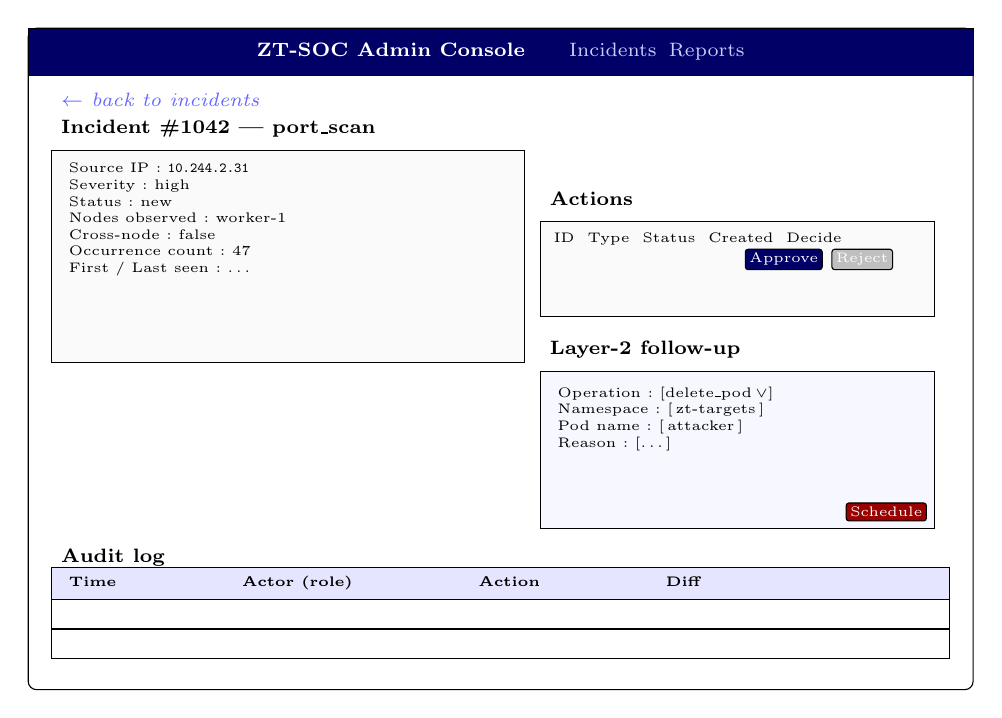
\begin{tikzpicture}[font=\scriptsize,
    win/.style ={draw, rounded corners=3pt},
    hbar/.style={draw, fill=blue!40!black, text=white, minimum height=0.6cm, align=left},
    panel/.style={draw, fill=gray!4},
    fld/.style ={draw, fill=white, minimum height=0.4cm},
    btn/.style ={draw, rounded corners=1pt, fill=blue!40!black, text=white, font=\tiny, inner sep=1.5pt},
  ]
  \node[win, minimum width=12cm, minimum height=8.4cm] (w) {};
  \node[hbar, anchor=north west, minimum width=12cm] at (w.north west)
    {\textbf{ZT-SOC Admin Console}\quad\quad \textcolor{blue!20}{Incidents}\;\;\textcolor{blue!20}{Reports}};
  \node[anchor=north west, font=\scriptsize\itshape, text=blue!60] at ([xshift=0.3cm,yshift=-0.7cm]w.north west) {$\leftarrow$ back to incidents};
  \node[anchor=north west, font=\scriptsize\bfseries] at ([xshift=0.3cm,yshift=-1.05cm]w.north west) {Incident \#1042 --- port\_scan};

  % Metadata table (2 cot)
  \node[panel, anchor=north west, minimum width=6.0cm, minimum height=2.7cm] (meta) at ([xshift=0.3cm,yshift=-1.55cm]w.north west) {};
  \node[anchor=north west, font=\tiny, align=left] at ([xshift=0.1cm,yshift=-0.05cm]meta.north west)
    {Source IP\ :\ \texttt{10.244.2.31}\\ Severity\ :\ high\\ Status\ :\ new\\ Nodes observed\ :\ worker-1\\ Cross-node\ :\ false\\ Occurrence count\ :\ 47\\ First / Last seen\ :\ \dots};

  % Actions table (ben phai metadata)
  \node[anchor=north west, font=\scriptsize\bfseries] at (0.5,2.25) {Actions};
  \node[panel, anchor=north west, minimum width=5.0cm, minimum height=1.2cm] (act) at (0.5,1.75) {};
  \node[font=\tiny, anchor=north west] at ([xshift=0.05cm,yshift=-0.03cm]act.north west) {ID \ Type \ Status \ Created \ Decide};
  \node[btn, anchor=north west] at ([xshift=2.6cm,yshift=-0.35cm]act.north west) {Approve};
  \node[btn, fill=gray!50, anchor=north west] at ([xshift=3.7cm,yshift=-0.35cm]act.north west) {Reject};

  % Layer-2 follow-up form
  \node[anchor=north west, font=\scriptsize\bfseries] at (0.5,0.35) {Layer-2 follow-up};
  \node[panel, fill=blue!3, anchor=north west, minimum width=5.0cm, minimum height=2.0cm] (fu) at (0.5,-0.15) {};
  \node[anchor=north west, font=\tiny, align=left] at ([xshift=0.1cm,yshift=-0.08cm]fu.north west)
    {Operation\ :\ [delete\_pod\,$\vee$]\\ Namespace\ :\ [\,zt-targets\,]\\ Pod name\ :\ [\,attacker\,]\\ Reason\ :\ [\dots]};
  \node[btn, fill=red!60!black, anchor=south east] at ([xshift=-0.1cm,yshift=0.1cm]fu.south east) {Schedule};

  % Audit log (duoi cung, ngang)
  \node[anchor=north west, font=\scriptsize\bfseries] at ([xshift=0.3cm,yshift=-6.5cm]w.north west) {Audit log};
  \node[draw, fill=blue!10, anchor=north west, minimum width=11.4cm, minimum height=0.4cm] (ah) at ([xshift=0.3cm,yshift=-6.85cm]w.north west) {};
  \node[font=\tiny\bfseries, anchor=west] at ([xshift=0.1cm]ah.west) {Time\hspace{1.6cm}Actor (role)\hspace{1.6cm}Action\hspace{1.6cm}Diff};
  \foreach \i in {0,1}{ \node[draw, fill=white, anchor=north west, minimum width=11.4cm, minimum height=0.38cm] at ([xshift=0.3cm,yshift={-7.25cm-\i*0.38cm}]w.north west) {}; }
\end{tikzpicture}
